\documentclass[tikz,border=0pt]{standalone}
\usetikzlibrary{calc}
% Palette: the 3D gym's colours (crates/core/src/mesh.rs, data/shaders/scene.frag).
\definecolor{sky}{HTML}{DCE6EE}
\definecolor{skyhi}{HTML}{F2F6F9}
\definecolor{wall}{HTML}{EDE6D3}
\definecolor{walldark}{HTML}{D6CCB4}
\definecolor{stripeblue}{HTML}{2F5CBF}
\definecolor{stripegold}{HTML}{F8C537}
\definecolor{window}{HTML}{CFE6FF}
\definecolor{windowlit}{HTML}{F6FBFF}
\definecolor{wood}{HTML}{DBA86B}
\definecolor{wooddark}{HTML}{B98549}
\definecolor{woodline}{HTML}{C9965A}
\definecolor{mat}{HTML}{2961CC}
\definecolor{matlit}{HTML}{4A82E8}
\definecolor{matdark}{HTML}{1C4597}
\definecolor{matseam}{HTML}{16377A}
\definecolor{red}{HTML}{DD3D38}
\definecolor{redlit}{HTML}{F06A5E}
\definecolor{reddark}{HTML}{A92A27}
\definecolor{yellow}{HTML}{F9C02E}
\definecolor{yellowlit}{HTML}{FFDB6B}
\definecolor{yellowdark}{HTML}{C9961C}
\definecolor{green}{HTML}{3FA866}
\definecolor{greenlit}{HTML}{62C98A}
\definecolor{greendark}{HTML}{2C7D4B}
\definecolor{pink}{HTML}{F27A93}
\definecolor{pinklit}{HTML}{F7A1B3}
\definecolor{orange}{HTML}{F28A2E}
\definecolor{orangelit}{HTML}{F7AE66}
\definecolor{orangedark}{HTML}{C2671A}
\definecolor{sky2}{HTML}{7FB8F0}
\definecolor{purple}{HTML}{8B5CC8}
\definecolor{skin}{HTML}{F2C49A}
\definecolor{skinlit}{HTML}{F8D8B8}
\definecolor{skindark}{HTML}{D9A47A}
\definecolor{skinb}{HTML}{B9835A}
\definecolor{skinbdark}{HTML}{93653F}
\definecolor{shirt}{HTML}{E2463F}
\definecolor{shirtdark}{HTML}{B23430}
\definecolor{shirtb}{HTML}{2F7DD8}
\definecolor{shirtbdark}{HTML}{225DA6}
\definecolor{shorts}{HTML}{21305A}
\definecolor{shortsdark}{HTML}{151F3D}
\definecolor{shoe}{HTML}{FFFFFF}
\definecolor{shoedark}{HTML}{D8DDE3}
\definecolor{hair}{HTML}{4A2F1C}
\definecolor{band}{HTML}{F8C537}
\definecolor{chick}{HTML}{FBE48F}
\definecolor{chicklit}{HTML}{FFF2BE}
\definecolor{chickdark}{HTML}{DCC064}
\definecolor{comb}{HTML}{E2302E}
\definecolor{beak}{HTML}{F28A2E}
\definecolor{noodle}{HTML}{57D163}
\definecolor{noodledark}{HTML}{3A9E45}
\definecolor{ball}{HTML}{D8302B}
\definecolor{balldark}{HTML}{A5211D}
\definecolor{balllit}{HTML}{F0645D}
\definecolor{duck}{HTML}{FFD12E}
\definecolor{duckdark}{HTML}{E0A814}
\definecolor{foam}{HTML}{2F6BE0}
\definecolor{foamdark}{HTML}{214FAD}
\definecolor{white}{HTML}{FFFFFF}
\definecolor{ink}{HTML}{1E2B45}
\definecolor{netline}{HTML}{9AA9BF}
\definecolor{glow}{HTML}{FFF4C2}
\begin{document}
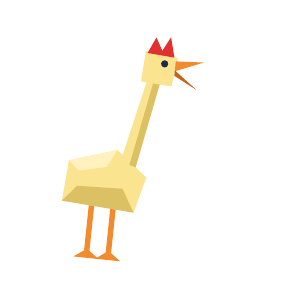
\begin{tikzpicture}[x=1cm,y=1cm]
\useasboundingbox (0,0) rectangle (3,3);
\begin{scope}[shift={(0.95,0.75)},scale=1.15,rotate=-6]
\fill[beak] (-0.15,-0.55) -- (-0.09,-0.55) -- (-0.09,0.1) -- (-0.15,0.1) -- cycle;
\fill[beak] (-0.26,-0.6) -- (0.02,-0.6) -- (-0.12,-0.5) -- cycle;
\fill[beak] (0.09,-0.55) -- (0.15,-0.55) -- (0.15,0.1) -- (0.09,0.1) -- cycle;
\fill[beak] (-0.02,-0.6) -- (0.26,-0.6) -- (0.12,-0.5) -- cycle;
\fill[chick] (-0.45,0) -- (0.35,-0.05) -- (0.45,0.35) -- (0.1,0.62) -- (-0.42,0.45) -- cycle;
\fill[chickdark] (-0.45,0) -- (0.35,-0.05) -- (0.2,0.2) -- (-0.3,0.18) -- cycle;
\fill[chicklit] (-0.42,0.45) -- (0.1,0.62) -- (0,0.42) -- (-0.3,0.35) -- cycle;
\fill[chick] (0.15,0.5) -- (0.32,0.45) -- (0.5,1.45) -- (0.36,1.48) -- cycle;
\fill[chickdark] (0.25,0.47) -- (0.32,0.45) -- (0.5,1.45) -- (0.43,1.47) -- cycle;
\fill[chick] (0.28,1.4) -- (0.62,1.38) -- (0.66,1.7) -- (0.3,1.74) -- cycle;
\fill[comb] (0.32,1.72) -- (0.4,1.9) -- (0.48,1.76) -- (0.56,1.92) -- (0.62,1.7) -- cycle;
\fill[beak] (0.64,1.55) -- (0.95,1.68) -- (0.64,1.66) -- cycle;
\fill[orangedark] (0.64,1.5) -- (0.9,1.37) -- (0.64,1.56) -- cycle;
\fill[ink] (0.52,1.62) circle (0.04);
\end{scope}
\end{tikzpicture}
\end{document}
